% BGIN Block 15 — the IKP co-chair's four sessions (15–16 Oct 2026, Georgetown University Capitol Campus)
% 1-4 / 1-7 PQC Migration (Room B, 15 Oct 09:50–13:00) · 2-6 Privacy Enhanced Authentication, ZKP & Proof of
% Personhood (Room B, 16 Oct 11:30–13:00) · 2-9 AML Policy, Forensics & Analytics — Common Taxonomy (FASE/IKP,
% Room A, 16 Oct 15:40–17:10, with Chloe White).
% House style of the GDC26 / Block 15 PQC decks: dark title bar, grey lead box, "Takeaway" line, BGIN mark in the footer.
% Facts follow the Block 15 programme (bgin-global.org/events/20261015-block15), bgin-global/pqc-agility-competition
% (draft v0, main 86c780a), the Block 14 meeting reports, the proof-of-human convergence note (Aug 2026) and the
% IKP KB in ~/BGIN_IKP. Everything shown is unratified.
% Build: latexmk -pdf Block15_IKP_CoChair_Sessions.tex
\documentclass[aspectratio=169,10pt]{beamer}
\usepackage[utf8]{inputenc}
\usepackage[T1]{fontenc}
\usepackage{helvet}
\renewcommand{\familydefault}{\sfdefault}
\usepackage{booktabs}
\usepackage{array}
\usepackage{graphicx}
\usepackage{fontawesome5}
\usepackage{tikz}
\usetikzlibrary{arrows.meta,positioning,calc}
\usepackage{qrcode}
\usepackage{hyperref}

\usetheme{default}
\setbeamersize{text margin left=7mm,text margin right=7mm}
\setlength{\tabcolsep}{4pt}
\definecolor{bar}{RGB}{25,25,29}
\definecolor{ink}{RGB}{35,35,40}
\definecolor{soft}{RGB}{110,110,118}
\definecolor{boxbg}{RGB}{242,242,244}
\definecolor{lane}{RGB}{225,227,232}
\definecolor{pqc}{RGB}{247,147,26}
\definecolor{pop}{RGB}{92,74,140}
\definecolor{popbg}{RGB}{236,233,244}
\definecolor{aml}{RGB}{18,108,108}
\definecolor{amlbg}{RGB}{228,240,239}
\setbeamercolor{normal text}{fg=ink}
\setbeamercolor{structure}{fg=bar}
\setbeamercolor{frametitle}{bg=bar,fg=white}
\setbeamercolor{block body}{bg=boxbg,fg=ink}
\setbeamercolor{pop body}{bg=popbg,fg=ink}
\setbeamercolor{aml body}{bg=amlbg,fg=ink}
\setbeamertemplate{navigation symbols}{}
\setbeamertemplate{itemize item}{\color{bar}\faAngleRight}
\setbeamertemplate{itemize subitem}{\color{soft}\textendash}
\setbeamertemplate{enumerate item}{\colorbox{bar}{\color{white}\scriptsize\insertenumlabel}}
\setbeamerfont{frametitle}{series=\bfseries,size=\large}
\setbeamertemplate{frametitle}{%
  \vskip-2pt\begin{beamercolorbox}[wd=\paperwidth,ht=8mm,dp=2.5mm,leftskip=6mm]{frametitle}%
  \usebeamerfont{frametitle}\insertframetitle\hfill{\small\mdseries\insertframesubtitle}\hspace{6mm}\end{beamercolorbox}}
\setbeamertemplate{footline}{%
  \begin{beamercolorbox}[wd=\paperwidth,ht=5mm,dp=2mm,leftskip=6mm,rightskip=6mm]{normal text}%
  \tiny\color{soft}\raisebox{-1.2pt}{
\includegraphics[height=3.2mm]{bgin_mark.png}}\hspace{1.2mm}%
  BGIN Block 15 --- IKP 1-7: PQC Migration (2)\hfill Washington, D.C. \textbar{} 15 Oct 2026, 11:30 / \insertframenumber\end{beamercolorbox}}
\newcommand{\takeaway}[1]{\par\vspace{1.5mm}{\small\color{bar}\faLink~\textbf{Takeaway:} #1}}
\newcommand{\lead}[1]{\begin{beamercolorbox}[wd=\textwidth,sep=2.5mm]{block body}\small #1\end{beamercolorbox}\par\vspace{2mm}}
\newcommand{\poplead}[1]{\begin{beamercolorbox}[wd=\textwidth,sep=2.5mm]{pop body}\small #1\end{beamercolorbox}\par\vspace{2mm}}
\newcommand{\amllead}[1]{\begin{beamercolorbox}[wd=\textwidth,sep=2.5mm]{aml body}\small #1\end{beamercolorbox}\par\vspace{2mm}}
\newcommand{\pillar}[3]{\begin{minipage}[t]{#1}\colorbox{bar}{\parbox{\dimexpr\linewidth-2\fboxsep}{\color{white}\small\textbf{#2}}}\par\vspace{1mm}{\small #3}\end{minipage}}
\newcommand{\cpillar}[4]{\begin{minipage}[t]{#2}\colorbox{#1}{\parbox{\dimexpr\linewidth-2\fboxsep}{\color{white}\small\textbf{#3}}}\par\vspace{1mm}{\small #4}\end{minipage}}
% \sectiontitle{accent}{kicker}{title}{subtitle}
\newcommand{\sectiontitle}[4]{{\setbeamertemplate{footline}{}\begin{frame}[plain]
  \begin{tikzpicture}[remember picture,overlay]
    \fill[bar] (current page.north west) rectangle (current page.south east);
    \node[anchor=north east,inner sep=0] at ([xshift=-7mm,yshift=-5mm]current page.north east){
\includegraphics[height=1.9cm]{bgin_logo.png}};
    \node[anchor=south west,text=#1,font=\small\bfseries] at ([xshift=7mm,yshift=-2.9cm]current page.north west){#2};
    \node[anchor=south west,text=white,font=\Large\bfseries,text width=13cm,align=left] at ([xshift=7mm,yshift=-4.7cm]current page.north west){#3};
    \node[anchor=north west,text=white,font=\small,text width=13cm,align=left] at ([xshift=7mm,yshift=-5.0cm]current page.north west){#4};
  \end{tikzpicture}
\end{frame}}}
\hypersetup{colorlinks,urlcolor=bar,linkcolor=ink}
\newcommand{\nohyph}{\hyphenpenalty=10000 \exhyphenpenalty=10000 \relax}

\begin{document}

% ================================================================ TITLE
{\setbeamertemplate{footline}{}
\begin{frame}[plain,t]
  \begin{tikzpicture}[remember picture,overlay]
    \fill[bar] (current page.north west) rectangle ([yshift=-3.5cm]current page.north east);
    \node[anchor=north east,inner sep=0] at ([xshift=-7mm,yshift=-5mm]current page.north east){
\includegraphics[height=1.9cm]{bgin_logo.png}};
    \node[anchor=west,text=white,font=\Large\bfseries,text width=11.2cm,align=left] at ([xshift=7mm,yshift=-1.35cm]current page.north west){PQC Migration (2) --- Crypto Agility as Governance; the NIST Path; the Decisions};
    \node[anchor=west,text=pqc,font=\small,text width=11.2cm,align=left] at ([xshift=7mm,yshift=-2.85cm]current page.north west){IKP session 1-7 \textperiodcentered{} Workshop W2 of the PQC Migration Prize series \textperiodcentered{} with NIST participation};
    \node[anchor=west,font=\normalsize,text width=13.2cm] at ([xshift=7mm,yshift=-4.6cm]current page.north west){Mitchell Travers (chair) \textperiodcentered{} Kanta Matsuura \textperiodcentered{} Tadahiko Itoh \textperiodcentered{} BGIN IKP Working Group};
    \node[anchor=north west,font=\small,text=soft,text width=13.2cm,align=left] at ([xshift=7mm,yshift=-5.0cm]current page.north west){BGIN Block \#15 \textbar{} Georgetown University Capitol Campus, Washington, D.C. \textbar{} 15 October 2026, Room B, 11:30--13:00 \textbar{} hybrid};
    \node[anchor=west,font=\scriptsize,text=soft,text width=13cm,align=left] at ([xshift=7mm,yshift=-6.5cm]current page.north west){The decisions session: seat the evaluation committee, take the scheme-scope rulings, move the metric register from v0 to v1 \textperiodcentered{} facts follow bgin-global/pqc-agility-competition, draft v0 \textperiodcentered{} ecosystem-neutral: no chain and no scheme is endorsed};
  \end{tikzpicture}
\end{frame}}

% ================================================================ CONTEXT
\begin{frame}{This Session --- What It Is For}
  \lead{Second IKP working session on the PQC Migration Prize --- the decisions session. Crypto agility as a governance property and the NIST PQC signature migration path across Bitcoin, Ethereum and other ecosystems. Block 15 is the second workshop (W2) of the six-month series on the pathway from competition to BGIN Standard to ISO/TC 307.}
  \begin{enumerate}\footnotesize\setlength{\itemsep}{0.5mm}
    \item Seating the evaluation committee (Phase A): nominations, conflict-of-interest disclosures, chairs
    \item Scheme-scope rulings for the testbed: ML-DSA, SLH-DSA, FN-DSA, XMSS, LMS and the classical baselines --- recorded as decision records
    \item Metrics register v0 $\rightarrow$ v1: consolidating the feedback from session 1-4
    \item Reference CPU class and reference transaction mix / block --- anchors for the performance metrics
    \item Whether consensus-layer and user-level evidence are scored on one rubric or two
    \item Proposed open-benchmark model for calibration tracks (decision record 0001)
    \item Pathway and next steps: testbed workshop (Nov), rubric, ``PQC-ready chain'' definition and call-text input package at the SSR co-located workshop (13 Dec, Baltimore), BGIN Standard outline (Feb 2027) toward ISO/TC 307
  \end{enumerate}
  \takeaway{Leave with a seated committee, a v1 metric register, scheme rulings on record, and named owners for the open questions --- not a locked migration spec.}
\end{frame}

% ================================================================ 11 agility
\begin{frame}{Session 1-7 --- Agility Is Harder Than Readiness}
  \lead{Evidence on the \textbf{mechanism of switching} --- hybrid and staged migration, scheme substitution cost, rollback, policy flexibility --- because the next migration is already certain and the primitive list will move again.}
  \begin{center}\scriptsize
  \begin{tabular}{@{}p{1.2cm}p{3.6cm}p{3.2cm}p{5.6cm}@{}}\toprule
    \textbf{Metric} & \textbf{What} & \textbf{Unit} & \textbf{How measured}\\ \midrule
    M-14 & Agility switch cost & time + coordination steps & scenario: swap scheme A to B under the proposed mechanism --- the core agility metric\\
    M-13 & Rollback cost & time + coordination steps & scenario: revert a staged migration\\
    M-12 & Migration throughput & keys / accounts per unit time & scenario; documents the user vs node-operator burden split\\
    M-21 & Legacy verification continuity & pass / fail + node cost & pre-migration signatures still verify after cutover\\
    M-20 & Governance fit & structured narrative & transition design, dormant assets, the owner-versus-attacker race --- recorded, not ruled\\ \bottomrule
  \end{tabular}
  \end{center}
  \takeaway{Agility written as a governance property is what lets the same rubric travel: competition $\rightarrow$ BGIN Standard $\rightarrow$ ISO/TC 307 $\rightarrow$ Japan's crypto-asset security criteria.}
\end{frame}

% ================================================================ 12 NIST path
\begin{frame}{The NIST Signature Migration Path --- What the Register Leans On}
  \lead{NIST is the algorithm and parameter authority for everything in scope; it is not a competition lane. Measurement-methodology cooperation is sought where appropriate, and NIST participation is invited in this session.}
  \begin{itemize}\small
    \item \textbf{FIPS 204 ML-DSA}, \textbf{FIPS 205 SLH-DSA} --- standardized; scheme rows S-01 and S-02.
    \item \textbf{FIPS 206 FN-DSA (Falcon)} --- draft; S-03 is confirmed at the scope ruling.
    \item \textbf{SP 800-208} XMSS and LMS / HSS --- stateful hash-based; S-04 and S-05 with state handling scored. Non-SP-800-208 parameterizations (hash-based aggregation with ZK-friendly hashes) need an explicit ruling.
    \item \textbf{ACVP / CAVP} wording is the correctness gate for calibration tracks.
    \item Hybrid / composite signatures follow the \textbf{IETF LAMPS} direction (C-01); the on-ramp signature candidates are \textbf{out of scope by gate G1}.
  \end{itemize}
  \takeaway{The register tracks NIST's list; it never extends it. When the list moves, the agility metrics are what say whether a stack can follow.}
\end{frame}

% ================================================================ 13 decisions
\begin{frame}{What Block 15 Decides --- the W2 Outputs}
  \begin{center}\scriptsize
  \begin{tabular}{@{}p{5.0cm}p{4.8cm}p{4.0cm}@{}}\toprule
    \textbf{Decision} & \textbf{Method} & \textbf{Lands as}\\ \midrule
    Committee seated (Phase A); chairs elected; second convener named & nominations + COI forms; formal vote & COMMITTEE.md roster\\
    OUTCOMES O1--O6 ratified (if not at W1) & formal vote, quorum of half & decisions/ record\\
    Metric register v0 $\rightarrow$ v1; directions per metric & rough consensus on the PR & evaluation/METRICS.md\\
    Scheme-scope rulings: C-01 hybrid, C-02 quantum-resistant output type as reference, S-04 non-SP-800-208 parameters, C-03 / C-04 / C-05 & formal vote per ruling & decisions/ records\\
    Open-benchmark model for calibration tracks & vote on decision 0001; recusals recorded & decisions/0001 accepted\\
    Open questions 1--6 assigned owners & conveners call it & workshop W2 record\\ \bottomrule
  \end{tabular}
  \end{center}
  \takeaway{Discuss on Discourse, record by pull request, rule by decision record. Every vote and every scope ruling gets an ADR. Nothing is final until the committee ratifies it and the host publishes the call.}
\end{frame}

% ================================================================ 14 open questions
\begin{frame}{The Open Questions That Need Owners Today}
  \begin{enumerate}\small
    \item Is the headline quantity \textbf{total overhead} or \textbf{migration speed}? The rubric decides the weights.
    \item Who must upgrade first --- \textbf{node operators or users} --- and how does M-12 reflect the burden split?
    \item How to score the \textbf{owner-versus-attacker race} during a migration window (M-20)?
    \item Which \textbf{reference CPU class} and \textbf{reference tx mix / block} anchor M-03 to M-09? Decision record 0002 territory, with $k$ and the tolerance band.
    \item Are \textbf{consensus-layer} (ETH-cons) and \textbf{user-level} (BTC-tx, ETH-user) evidence scored on one rubric or two?
    \item For each metric, which attack class --- \textbf{on-spend, at-rest, on-setup} --- does it defend against?
  \end{enumerate}
  \par\vspace{1mm}
  {\small Also for the room: what the \emph{``PQC-ready chain'' definition} has to contain for M-22 to be scorable by December; and whether the ECDSA.fail public-note discipline (model and harness named, re-run by a validator) is the admission rule for agent-produced numbers.}
\end{frame}

% ================================================================ 15 timeline
\begin{frame}{From This Room to the 2028 Award}
  \begin{center}
  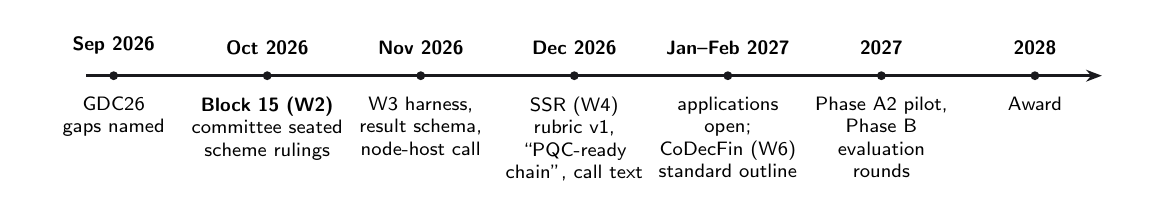
\begin{tikzpicture}[font=\scriptsize]
    \draw[line width=1pt,bar,-{Stealth[length=2mm]}] (0,0) -- (12.9,0);
    \foreach \x/\lab/\txt in {
      0.35/Sep 2026/{GDC26\\ gaps named},
      2.3/Oct 2026/{\textbf{Block 15 (W2)}\\ committee seated\\ scheme rulings},
      4.25/Nov 2026/{W3 harness,\\ result schema,\\ node-host call},
      6.2/Dec 2026/{SSR (W4)\\ rubric v1, ``PQC-ready\\ chain'', call text},
      8.15/Jan--Feb 2027/{applications open;\\ CoDecFin (W6)\\ standard outline},
      10.1/2027/{Phase A2 pilot,\\ Phase B evaluation\\ rounds},
      12.05/2028/{Award}}
      {\fill[bar] (\x,0) circle (1.6pt);
       \node[above=1.5mm,align=center,font=\scriptsize\bfseries] at (\x,0) {\lab};
       \node[below=1.5mm,align=center,text width=1.95cm] at (\x,0) {\txt};}
  \end{tikzpicture}
  \end{center}
  \par\vspace{1mm}
  \begin{center}\small
    Competition / evaluation $\rightarrow$ BGIN Standard $\rightarrow$ ISO/TC 307 $\rightarrow$ Japan's crypto-asset security criteria
  \end{center}
  {\scriptsize\color{soft} Dates are indicative until the host confirms the call. SSR 2026 PQC-for-blockchains workshop: Sun 13 Dec, Baltimore; peer-reviewed papers there are intended to be reflected in the competition specification.}
  \takeaway{This morning can still change what the call asks teams to prove. SSR on 13 December is the next drafting stop.}
\end{frame}

% ================================================================ ENGAGE
\begin{frame}{How to Engage}
  \begin{columns}[T]
    \begin{column}{0.55\textwidth}
      \begin{itemize}\small
        \item \textbf{Evaluation committee} --- nominate via the issue template; seats are individuals with COI disclosure, not projects.
        \item \textbf{Second convener} --- the record cannot move on one signing key; a second convener with a key restores the approval rule.
        \item \textbf{Testbed node host} --- a university or neutral lab; the call opens at W3 (November); hosting is separated from judging.
        \item \textbf{SSR workshop, 13 Dec} --- rubric v1, the ``PQC-ready chain'' definition, and the call-text input package.
        \item \textbf{Submit / build} --- when the official call opens (planned 2027).
      \end{itemize}
    \end{column}
    \begin{column}{0.42\textwidth}
      \begin{center}\tiny
        \begin{tabular}{@{}>{\centering\arraybackslash}p{1.85cm}@{\hspace{1mm}}>{\centering\arraybackslash}p{1.85cm}@{\hspace{1mm}}>{\centering\arraybackslash}p{1.85cm}@{}}
          \qrcode[height=1.35cm]{https://bgin-global.org/events/20261015-block15/sessions/1-7} &
          \qrcode[height=1.35cm]{https://github.com/bgin-global/pqc-agility-competition} &
          \qrcode[height=1.35cm]{https://bgin.discourse.group/c/post-quantum-crypto-agility-competition/44} \\[0.5mm]
          \textbf{This session} & \textbf{Repository} & \textbf{Discourse category} \\
          bgin-global.org/events/ 20261015-block15/sessions/1-7 & github.com/bgin-global/ pqc-agility-competition & bgin.discourse.group/c/ post-quantum-crypto-agility-competition/44
        \end{tabular}
      \end{center}
    \end{column}
  \end{columns}
  \takeaway{Discuss on Discourse, record by pull request, rule by decision record. Every vote and every scope ruling gets an ADR.}
\end{frame}

% ================================================================ CLOSE
{\setbeamertemplate{footline}{}
\begin{frame}[plain]
  \begin{tikzpicture}[remember picture,overlay]
    \fill[bar] (current page.north west) rectangle (current page.south east);
    \node[anchor=south,text=white,font=\Large\bfseries,text width=13.5cm,align=center,execute at begin node=\nohyph] at ([yshift=6mm]current page.center){Agility is harder than readiness, and it is what future-proofs the system.};
    \node[anchor=north,text=white,font=\small,text width=13.5cm,align=center,execute at begin node=\nohyph] at ([yshift=3mm]current page.center){The register tracks NIST's list; it never extends it. When the list moves, the agility metrics are what say whether a stack can follow.};
    \node[anchor=north,text=soft,font=\small,text width=13.5cm,align=center,execute at begin node=\nohyph] at ([yshift=-9mm]current page.center){BGIN IKP Working Group \textperiodcentered{} Post-Quantum Crypto Agility Competition category on the BGIN Discourse \textperiodcentered{} github.com/bgin-global/pqc-agility-competition};
    \node[anchor=south east,inner sep=0] at ([xshift=-7mm,yshift=5mm]current page.south east){
\includegraphics[height=1.4cm]{bgin_logo.png}};
  \end{tikzpicture}
\end{frame}}

\end{document}
